\section{ADDITIONAL EXPERIMENTS}\label{sec:add_expes}

\subsection{Details of \textsf{glmnet} versus \textsf{SLOPE} Comparison}
\label{sec:slope-vs-glmnet}

In this experiment, we ran the \pkg{glmnet}~\parencite{friedman2022} and \pkg{SLOPE}~\parencite{larsson2022d} packages on the \dataset{bcTCGA} dataset, selecting the regularization sequence \(\lambda\) such that there were 100 nonzero coefficients and clusters at the optimum for \pkg{glmnet} and \pkg{SLOPE} respectively.
We used a duality gap of \(10^{-6}\) as stopping criteria.
The features were centered by their means and scaled by their standard deviation.
The code is available in the supplement.

\subsection{Study on Proximal Gradient Descent Frequency}
To study the impact of the frequence at which the pgd step in the \texttt{hybrid} solver on the speed of the algorithm, we performed a comparative study using the \dataset{rcv1} dataset. 
We set the value of this parameter to value ranging from $1$ \textit{i.e.}, \texttt{pgd} algorithm, to 9 meaning that a pgd step is taken every $9$ epochs. 
The sequence of $\lambda$ has been set with the Benjamini-Hochberg method and parametrized with $0.1 \lambda_{\text{max}}$. 

\Cref{fig:pgd_freq} shows the suboptimality score as a function of the time for the different values of the parameter controlling the frequency at which a pgd step is going to be taken. 
A first observation is that as long as this parameter is greater than $1$ meaning that we perform some coordinate descent steps, we can see a significant speed-up. 
For all our experiments, this parameter was set to $5$ and was never changed. 
We see on this figure that any choice of parameter between $3$ and $9$ would basically lead to the same performance. 

\begin{figure*}[htb]
  \centering
  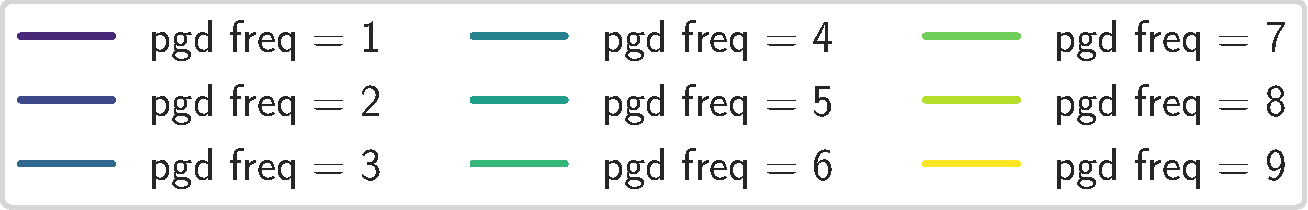
\includegraphics[scale=0.47]{pgd_freq_legend.pdf}
  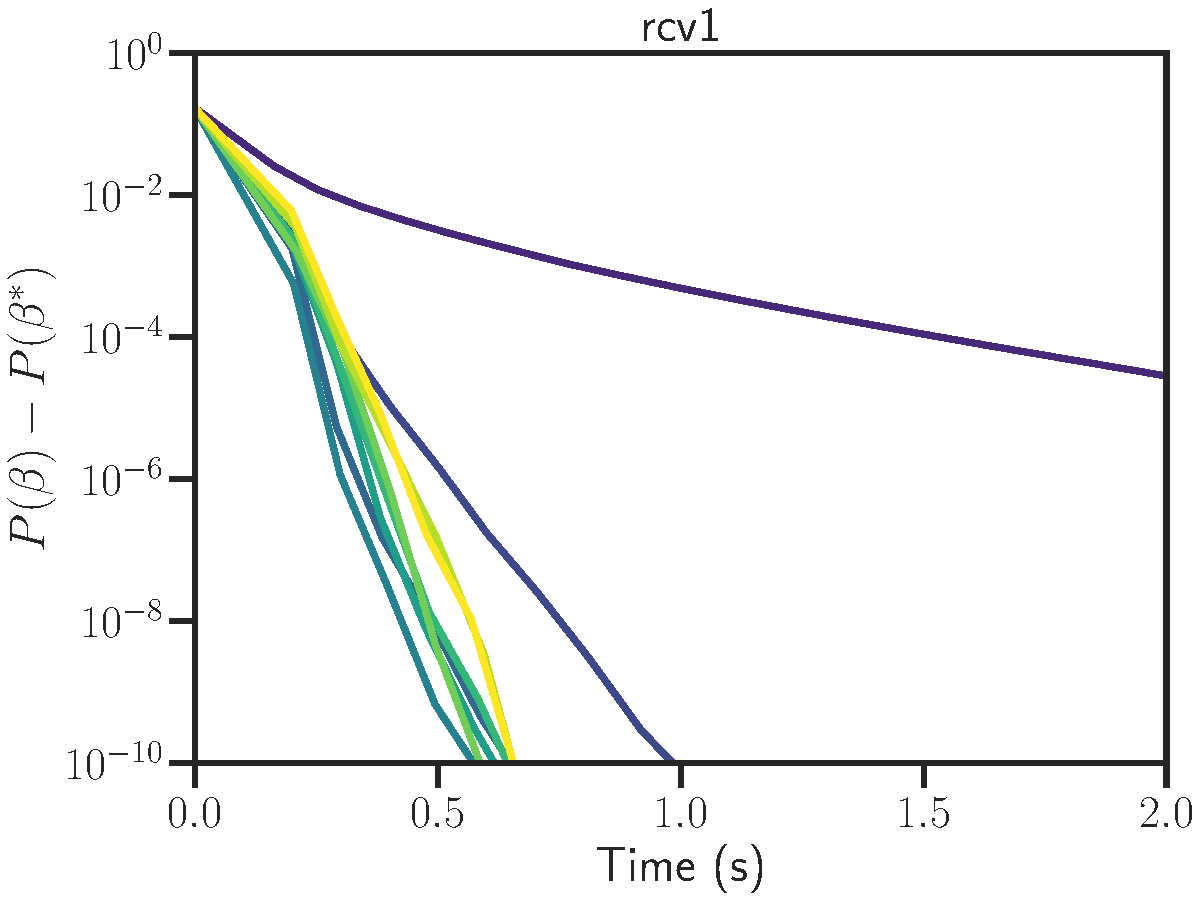
\includegraphics[scale=0.5]{pgd_freq.pdf}
  \caption{Suboptimality score as a function of the time for different frequency of pdg step inside the \texttt{hybrid} solver.}
  \label{fig:pgd_freq}
\end{figure*}
